\subsection{RSS3 \glsfmtfull{GI}}
\label{subsec:GI}

{
    \begin{figure}[tb!]
        \centering
        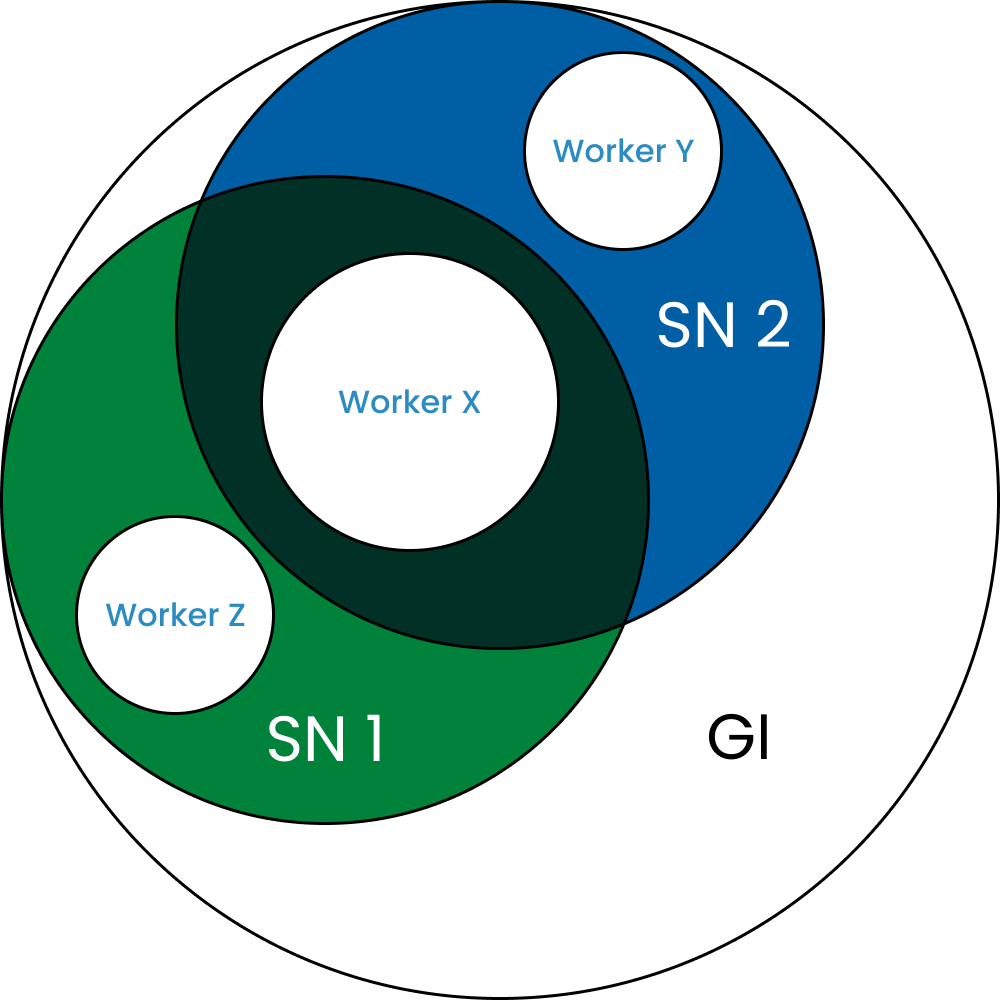
\includegraphics[width=0.7\columnwidth]{figures/GI.png}
        \caption{A Venn diagram illustrating the relationship between the worker, the \glsfmtlong{Node}, and the \glsfmtlong{GI}.}
        \label{fig:GI}
    \end{figure}
}

\glspl{GI} are responsible for facilitating coordination among \glspl{Node} and engaging with the \gls{VSL} and perform critical duties to ensure the \gls{DSL} is robust and reliable.

Given the importance of the \glspl{GI} to the Network, their operation is subject to a set of stringent requirements imposed by the Network.

{
    \begin{figure}[tb!]
        \centering
        \includegraphics[width=0.7\columnwidth]{figures/GI-components.png}
        \caption{The core components of \gls{GI}.}
        \label{fig:GI-components}
    \end{figure}
}

\subsubsection{Broadcaster and Enforcer}
The broadcaster and enforcer components of the \gls{GI} function as regulatory mechanisms for \glspl{Node}, ensuring the maintenance of service quality. The broadcaster continuously monitors the status of all \glspl{Node} to identify any unusual behavior. Given the permissionless nature of the \gls{DSL}, robust quality assurance is essential to maintain the integrity and reliability of the \glsfmtlong{R3N}.
The enforcer, in collaboration with the broadcaster and router, maintains a comprehensive record of demotions and slashing events, and implements measures to encourage \glspl{Node} to meet the established requirements.

\subsubsection{Indexer}
The indexer component is tasked with the systematic structuring of activities occurring across the entire Network. It subsequently provides this structured information through a network transparency API, facilitating comprehensive insight into Network operations.

\subsubsection{Payment Processor}
The payment processor, operating in conjunction with the settler, ensures the accurate distribution of collected request fees to the corresponding \glspl{Node} and content creators.
Furthermore, the payment processor calculates the Network's average tax rate and updates the settlement contract on the \gls{VSL} accordingly, maintaining financial balance within the system.

\subsubsection{Router}
The router component of the \gls{GI} is responsible for ensuring that requests are routed and served with optimal performance and minimal latency.
The distinctive architecture of the \gls{DSL} necessitates that the \gls{GI} be equipped with enhanced computational capabilities to determine the most efficient routing path for incoming requests. Typically, a request retrieves \glsfmtlong{OI} from either a single \gls{Node} or, more frequently, from a distributed group of \glspl{Node} concurrently.

\subsubsection{Settler}
The settler component of the \gls{GI} initiates the submission of \glspl{Node}' work records to the \gls{VSL}. Subsequently, the settlement contract on the \gls{VSL} verifies these records and facilitates the distribution of network rewards, ensuring fair compensation for network participants.

\subsection{Reliability Score}

A \gls{GI} routes requests to \glspl{Node} based on their information coverage and a \gls{RS}.
The calculation of \reliabilityScore\ is based on a range of factors, including but not limited to the \gls{Node}'s uptime, work, slash records, operation deposit, and staking/trust pool size.
\glspl{Node} with a higher \reliabilityScore\ have an increased likelihood of receiving requests.
